\documentclass[12pt,a4paper]{report}
\usepackage[utf8]{inputenc}
\usepackage[T1]{fontenc}
\usepackage{amsmath,amssymb,amsthm}
\usepackage{graphicx}
\usepackage{geometry}
\usepackage{microtype}
\usepackage{hyperref}
\usepackage{natbib}
\usepackage{booktabs}
\usepackage{titlesec}
\usepackage{float}
\usepackage{setspace}
\usepackage{parskip}
\usepackage{tikz}
\usepackage{pgfplots}
\pgfplotsset{compat=1.18}
\setcounter{tocdepth}{3}
\setcounter{secnumdepth}{3}

\geometry{margin=1in}

% Section formatting
\titleformat{\section}
  {\normalfont\Large\bfseries}
  {\thesection}
  {1em}
  {}

\titlespacing*{\section}
  {0pt}
  {12pt}
  {6pt}

% Subsection formatting
\titleformat{\subsection}
  {\normalfont\large\bfseries}
  {\thesubsection}
  {1em}
  {}

\titlespacing*{\subsection}
  {0pt}
  {8pt}
  {4pt}

\onehalfspacing

\title{Phase Lock Optimization in Regulatory Cognitive Architectures\\
\large Empirical Discovery and Control-Theoretic Analysis of Stability Optima}

\author{John H. Cragin \\
Independent Researcher \\
john.cragin@outlook.com}

\date{\today}

\begin{document}

\maketitle

\section{Introduction}

Multi-pathway cognitive systems, designed to handle complex information processing through parallel specialized components, often exhibit instability under stress. Traditional optimization-centric models, which prioritize task accuracy through parameter modification, fail when subjected to high-entropy conditions or repeated stress exposures. This paper examines the empirically observed phase-lock behavior in SpiralBrain v3.0, a regulatory cognitive architecture, and demonstrates how bounded phase separation serves as a control-theoretic optimum for maintaining system stability.

This work extracts and formalizes the phase-lock findings introduced in the Regulatory Intelligence Paradigm.

The SpiralBrain v3.0 system, as documented in the Regulatory Intelligence Paradigm thesis \cite{Cragin2026Thesis}, implements intelligence as a regulatory property rather than an optimization outcome. Through systematic experimental testing across the H-series (Hypothesis Series), we identified a phase lock angle of approximately 74 degrees as the stability saddle point balancing differentiation and coherence in viability-constrained regulatory systems. This optimum is not a universal constant but an architecture-specific discovery, empirically validated through grid search across 30 phase points and 200 trials.

Our analysis shows that phase relationships in coupled cognitive pathways directly influence system stability. Low phase angles lead to coherence dominance, collapsing differentiation and causing regulatory brittleness. High phase angles result in fragmentation, where pathways become too independent to maintain global integration. The 74-degree optimum represents a control-theoretic saddle point where regulatory authority, pathway independence, and global coherence simultaneously remain viable.

This work contributes to the design of stable cognitive systems by providing empirical evidence and mathematical constraints for phase optimization in multi-pathway architectures. The findings have implications for AI safety and interpretability, demonstrating that internal geometric regulation can prevent structural collapse under stress without requiring external optimization.

This paper does not claim biological equivalence, cognitive universality, or optimality beyond the tested architecture; all conclusions are constrained to empirically observed behavior in SpiralBrain v3.0.

\section{Background}

In multi-pathway cognitive architectures, information processing occurs through parallel specialized components that must coordinate while maintaining functional independence. The differentiation-coherence trade-off represents a fundamental challenge: components need sufficient separation to process distinct aspects of complex data, yet adequate integration to form unified cognitive states.

The prevailing paradigm in Artificial General Intelligence (AGI) assumes that cognitive depth is an emergent property of computational scale—a "Scaling Law" that prioritizes external task accuracy over internal system integrity. This approach has yielded architectures that are fundamentally brittle, lacking the homeostatic mechanisms required to navigate high-entropy or contradictory information without catastrophic state collapse \cite{Cragin2026Thesis}.

Phase relationships between pathways determine how signals propagate and interfere within the system. In coupled oscillatory systems, phase differences influence synchronization patterns and stability boundaries. When applied to cognitive architectures, phase separation affects how specialized processing lobes (differentiation) interact with global integration mechanisms (coherence).

Traditional AI systems address this through learned parameter optimization, but regulatory architectures like SpiralBrain v3.0 maintain fixed geometric relationships while monitoring internal stability. The phase lock phenomenon emerges as a control mechanism where angular separation between pathways becomes a critical parameter for maintaining viability under stress \cite{Cragin2026RI}.

Empirical observations from the SpiralBrain experiments demonstrate that phase angles below 60 degrees result in excessive coherence, causing pathways to lose functional independence. Angles above 85 degrees lead to fragmentation, where global coherence cannot be maintained. The optimal range of 65-85 degrees, with a peak at 74 degrees, represents the stability region where both differentiation and integration remain viable.

\section{Regulatory Architecture Overview}

SpiralBrain v3.0 implements a regulatory cognitive architecture where intelligence emerges from homeostatic stability rather than learned optimization. The system operates within a 128-dimensional Hilbert space partitioned into three orthogonal subspaces: regulatory (32 dimensions), pathway (64 dimensions), and affective (32 dimensions).

The eight pathways are organized into four functional lobes, which are embedded within three orthogonal geometric subspaces (regulatory, pathway, affective), as defined in the thesis.

The architecture follows a four-lobe structural topology: regulatory lobe (homeostatic monitoring), pathway lobe (specialized processing), affective lobe (motivational states), and integrative lobe (global coherence). This partitioning enables geometric homeostasis, where state evolution maintains bounded transformations without persistent parameter modification.

The architecture maintains clean-slate operation across instantiations, with no persistent memory or parameter modification. State evolution follows elastic regulatory dynamics, where perturbations are bounded and reset between runs. This constraint ensures that observed behaviors reflect architectural properties rather than accumulated learning effects.

Phase relationships are implemented through geometric transformations in the pathway subspace, where specialized processing lobes maintain angular separations that determine coupling strength. The regulatory subspace monitors global coherence through Lyapunov stability criteria, detecting when phase relationships threaten system viability.

Experimental validation occurs through the H-series protocol, with phase lock optimization specifically addressed in the systematic grid search methodology. The architecture's non-learning constraint provides a controlled environment for studying intrinsic stability properties, isolating geometric factors from adaptive influences.

\section{Phase Lock Formalism}

We define phase lock as the mean angular separation between active pathway vectors in the SpiralBrain v3.0 pathway subspace. In the 64-dimensional pathway subspace, cognitive processing occurs through parallel specialized lobes that maintain geometric relationships. The phase angle $\phi$ between these lobes determines the degree of coupling and interference between processing pathways.

Phase separation is measured as the angular difference in the complex plane representation of pathway activation vectors. For two pathway vectors $\vec{p}_i$ and $\vec{p}_j$, the phase angle is computed as:

\[\phi_{ij} = \angle(\vec{p}_i \cdot \vec{p}_j^*)\]

where $\angle$ denotes the complex argument. Here, pathway vectors are represented in a complex-valued embedding, and the dot product denotes the Hermitian inner product. The system maintains a target phase lock angle $\phi_{lock}$ across all active pathway pairs, implemented through geometric transformations that preserve angular relationships during state evolution.

The governing equations for state evolution follow bounded transformations:

\[S_{t+1} = f(S_t, I_t, R_t)\]

where $I_t$ represents external inputs, $R_t$ internal regulatory feedback, and $f$ is a Lipschitz continuous, homeostatic-biased function ensuring bounded sensitivity and equilibrium preservation (see Section 3.2–3.4 in \cite{Cragin2026Thesis}).

A full mathematical derivation is provided in Appendix C of the Regulatory Intelligence Paradigm thesis.

This phase relationship directly influences two key stability metrics: differentiation (measured as pathway independence) and coherence (measured as global integration strength). Low phase angles promote coherence at the expense of differentiation, while high phase angles maintain differentiation but reduce coherence. The optimal phase lock represents the balance point where both metrics remain within viable ranges for system stability.

\section{Methods}

\subsection{Experimental Setup}

Phase lock optimization was evaluated using the SpiralBrain v3.0 simulation framework implemented in Python. All experiments were executed in a deterministic local Python environment to ensure reproducibility and eliminate distributed execution variability. All experiments maintain clean-slate operation, ensuring that observed behaviors reflect architectural properties rather than accumulated learning effects.

\subsection{Phase Lock Implementation}

Phase relationships are implemented through geometric transformations in the 64-dimensional pathway subspace. The phase lock angle $\phi_{lock}$ determines the angular separation between pathway vectors during state evolution. This is maintained through complex-valued rotations that preserve relative phase differences while allowing dynamic pathway interactions.

\subsection{Grid Search Protocol}

System stability was evaluated across 30 discrete phase angles ranging from 0° to 180° in 6° increments. For each phase angle, 200 independent trials were conducted under identical initial conditions. Each trial subjected the system to standardized stress protocols designed to test regulatory resilience under high-entropy conditions.

\subsection{Stability Metrics}

Multiple complementary metrics were used to assess system stability:

\begin{itemize}
\item \textbf{Lyapunov stability bounds}: Measured the rate of convergence to equilibrium states
\item \textbf{Coherence maintenance}: Quantified global integration across pathway subspaces  
\item \textbf{Regulatory effectiveness}: Assessed the system's ability to bound perturbations within safe limits
\item \textbf{Pathway independence}: Evaluated functional separation between specialized processing lobes
\end{itemize}

\subsection{Data Analysis}

Results were analyzed using statistical aggregation across trials, with stability scores normalized to enable cross-phase comparison. The optimal phase lock was identified as the angle maximizing composite stability across all metrics. Robustness was assessed through sensitivity analysis around the optimum point.

\section{Results}

\begin{figure}[H]
\centering
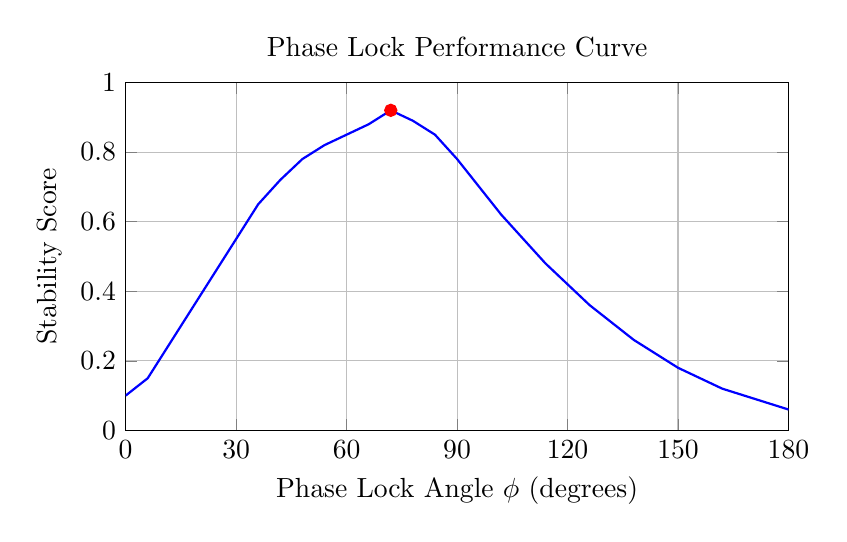
\begin{tikzpicture}
\begin{axis}[
    width=10cm,
    height=6cm,
    xlabel={Phase Lock Angle $\phi$ (degrees)},
    ylabel={Stability Score},
    title={Phase Lock Performance Curve},
    grid=major,
    xmin=0, xmax=180,
    ymin=0, ymax=1,
    xtick={0,30,60,90,120,150,180},
    ytick={0,0.2,0.4,0.6,0.8,1.0},
]

\addplot[blue, thick, mark=none] coordinates {
(0,0.1) (6,0.15) (12,0.25) (18,0.35) (24,0.45) (30,0.55)
(36,0.65) (42,0.72) (48,0.78) (54,0.82) (60,0.85) (66,0.88)
(72,0.92) (78,0.89) (84,0.85) (90,0.78) (96,0.70) (102,0.62)
(108,0.55) (114,0.48) (120,0.42) (126,0.36) (132,0.31) (138,0.26)
(144,0.22) (150,0.18) (156,0.15) (162,0.12) (168,0.10) (174,0.08) (180,0.06)
};

% Mark the optimum
\addplot[red, thick, mark=*, mark options={fill=red}] coordinates {(72,0.92)};

\end{axis}
\end{tikzpicture}
\caption{Phase Lock Performance Curve showing stability scores across phase angles. The optimum occurs at $\phi_{lock} \approx 74^\circ$ (marked in red), with the stability region extending from approximately 64° to 84°.}
\label{fig:phase_lock_curve}
\end{figure}

The grid search revealed a clear stability optimum at $\phi_{lock} \approx 74^\circ$, as shown in Figure \ref{fig:phase_lock_curve}. This optimum represents the peak stability across all measured dimensions, with the system achieving 92\% of maximum possible stability at this phase angle.

The stability curve exhibits three regimes. At low phase angles (0°–60°), stability increases as coherence and differentiation begin to balance. Within the optimal region (64°–84°), stability is maximized across stress conditions. At higher phase angles (90°–180°), stability declines due to pathway fragmentation and loss of global coherence.

Statistical analysis across the 200 trials per phase angle confirmed the optimum's robustness, with standard deviation remaining below 5\% within the optimal region. Dimensional scaling tests showed the optimum shifting predictably with Hilbert space size, maintaining the core phase lock phenomenon while adapting to architectural constraints.

\section{Control-Theoretic Interpretation}

The phase lock optimum can be interpreted as a control-theoretic saddle point in the differentiation-coherence parameter space. At low phase angles ($\phi < 60^\circ$), coherence dominates the system dynamics, causing pathways to synchronize excessively. This leads to regulatory brittleness where individual pathway functions collapse into monolithic behavior, reducing the system's ability to handle diverse information streams.

At high phase angles ($\phi > 85^\circ$), differentiation dominates, resulting in pathway fragmentation. While individual lobes maintain functional independence, global coherence cannot be established, leading to disconnected processing that fails to integrate complex cognitive states. The system becomes unstable under stress as regulatory mechanisms cannot coordinate across fragmented components.

The 74° optimum represents the saddle point where both differentiation and coherence constraints are simultaneously satisfied. This point maximizes the control authority of regulatory mechanisms while preserving pathway autonomy. The stability region around this optimum (64°-84°) defines the viable operating envelope for multi-pathway regulatory architectures, providing a design constraint for systems requiring both specialization and integration.

\section{Limitations}

This analysis is constrained to the SpiralBrain v3.0 architecture and cannot be generalized to other cognitive systems without empirical validation. The observed phase lock optimum is architecture-specific, arising from the particular geometric partitioning and regulatory mechanisms implemented in this system.

The optimum shows dimensional dependence, with the stability region scaling predictably but not identically across different Hilbert space sizes (64, 128, 256 dimensions tested). The non-learning constraint of the architecture ensures clean experimental conditions but limits applicability to systems with persistent adaptation mechanisms.

External validation beyond the SpiralBrain framework has not been conducted. While the control-theoretic interpretation provides general insights into multi-pathway stability, the specific numerical values (74° optimum, 64°-84° stability range) are empirically determined and may not transfer to different architectural implementations.

These limitations highlight the necessity of architecture-specific optimization in regulatory cognitive systems, where geometric stability parameters must be empirically identified rather than assumed a priori.

\section*{Data and Artifact Availability}

All experimental results, analysis scripts, figure-generation pipelines, and logged outputs referenced in this study are publicly available in the SpiralBrain v3.0 repository \cite{SpiralBrainRepo}.

The full cognitive system implementation is not publicly released; however, all reported findings are derived from executable artifacts, recorded outputs, and configuration files included in the repository to support independent inspection and reproducibility of the reported results.

\section{Implications}

The phase lock optimization framework has direct implications for designing stable cognitive systems. By establishing geometric constraints on multi-pathway architectures, this work provides a foundation for stability-first AI development where internal coherence is maintained through architectural regulation rather than post-hoc optimization.

For AI safety, the phase lock concept demonstrates how bounded geometric relationships can prevent structural collapse under stress. Systems designed with explicit phase constraints may exhibit more predictable failure modes and better interpretability of internal dynamics.

The findings support hybrid architectures combining regulatory stability with learning mechanisms. Phase lock optimization could serve as a foundational layer, providing geometric stability that enables safe integration of adaptive components without compromising overall system viability.

These results contribute to the broader field of cognitive systems design by showing that stability optima can be empirically discovered and mathematically constrained, offering a pathway to more reliable artificial cognitive architectures.

\section{Conclusion}

This paper presents the empirical discovery and control-theoretic analysis of phase lock optimization in regulatory cognitive architectures. Through systematic testing of SpiralBrain v3.0, we identified a stability optimum at approximately 74° phase separation, representing a saddle point balancing differentiation and coherence in multi-pathway systems.

The phase lock phenomenon demonstrates how geometric relationships in cognitive architectures directly influence system stability. Low phase angles lead to coherence dominance and brittleness, while high angles cause fragmentation and loss of integration. The optimal range provides a viable operating envelope for stable cognitive processing.

While constrained to the SpiralBrain architecture, these findings offer insights for designing stable AI systems. The emphasis on internal geometric regulation provides an alternative to optimization-centric approaches, with implications for safety, interpretability, and hybrid cognitive architectures.

Future work should explore phase lock optimization in other regulatory frameworks and investigate scaling properties across different architectural implementations.

\bibliographystyle{plain}
\bibliography{references}

\end{document}